\documentclass[aspectratio=169]{ctexbeamer}
\usepackage{tikz}
\usepackage{pgfplots}
\usetikzlibrary{calc}
\usepackage{amssymb,amsmath}
\usepackage{enumitem}
\usepackage{geometry}
%\geometry{paperwidth=200mm}
\pgfplotsset{compat=1.18}
\usetheme{Madrid} %Madrid,蓝色调为主。
\usecolortheme{beaver} %beaver
\usefonttheme{professionalfonts}

\date{\today}
\begin{document}
\begin{frame}[t]{数学课程的总目标}
\begin{spacing}{1.5} %设置1.5倍行距
{\Large
通过义务教育阶段的数学学习,学生逐步:\\
\begin{enumerate}[label={\arabic*.}]
\item \textbf{会用数学的眼光观察现实世界;}\\
\item \textbf{会用数学的思维思考现实世界;}\\
\item \textbf{会用数学的语言表达现实世界。}\\
\end{enumerate}
(简称“三会”) 。\\
}
\end{spacing}
\end{frame}

\begin{frame}[t]{数学考试丢分的四大原因}
\begin{spacing}{1.5} %设置行距
{\Large
数学考试丢分的四大根本原因:\\
\begin{enumerate}[label={\arabic*.}]
\item \textbf{知识点不透彻;}\\
\item \textbf{题型不熟练;}\\
\item \textbf{计算不准确;}\\
\item \textbf{计算速度慢。} \\
\end{enumerate}
(简称“四因”) 。\\
}
\end{spacing}
\end{frame}

\begin{frame}[t]{学好数学的五个步骤}
\begin{spacing}{1.2} %设置行距
{\Large
学好数学的五个步骤:\\
\begin{enumerate}[label={\arabic*.}]
\item \textbf{发现个案(发现有趣的个案);}\\
\item \textbf{类似案例(寻找类似的案例);}\\
\item \textbf{总结规律(找到一般的规律:从特殊到一般);}\\
\item \textbf{定义证明(给出定义或证明)。} \\
\item \textbf{实际应用(应用到实践中去:从一般到特殊)。} \\
\end{enumerate}
(简称“五步骤”) 。\\
\alert{第一步到第三步:大胆假设;第四步:小心求证;第五步:放心应用。}
}
\end{spacing}
\end{frame}
% 有理数的引入
\begin{frame}{1.1 有理数的引入}
\begin{definition}
\textbf{\textcolor{orange}{正整数、0 和负整数统称为整数(integer), 正分数和负分数统称为分数(fraction).\\
整数和分数统称为有理数(rational number).}}
\end{definition}
\begin{columns}
\column{0.5\textwidth}
\[
\mbox{有理数}\begin{cases}
\mbox{整数} \begin{cases}
    \mbox{正整数} \\
    0 \\
    \mbox{负整数}
    \end{cases} \\
\mbox{分数}  \begin{cases}
    \mbox{正分数} \\
    \mbox{负分数}
    \end{cases}
\end{cases}
\]

\column{0.5\textwidth}
\[
\mbox{小数}\begin{cases}
\mbox{有限小数} \\
\mbox{无限小数} \begin{cases} 
\mbox{无限循环小数} \\
\mbox{无限不循环小数}
\end{cases}
\end{cases}
\]

\end{columns}
\vspace{12pt}
\alert{\textbf{0既不是正数,也不是负数,是正数与负数的分界点。}} \\
\alert{\textbf{有限小数和无限循环小数是分数,无限不循环小数不是分数。}} \\
\textbf{思考:无限不循环小数是什么数?}
\end{frame}

%小数如何转化为分数
\begin{frame}{小数如何转化为分数}
有限小数如何转化为分数:\\
\[0.245=\dfrac{245}{1000}=\dfrac{49}{200}
\]
无限循环小数如何转化为分数?【华东师范大学七年级上册(2024)P73】
%循环节的小圆点表示\dot{x}
\begin{align*}
1000\times 0.\dot{2}4\dot{5} &= 245.\dot{2}4\dot{5} = 245 + 0.\dot{2}4\dot{5} \\
999 \times 0.\dot{2}4\dot{5} &= 245 \\
0.\dot{2}4\dot{5} &= \dfrac{245}{999}
\end{align*}
\end{frame}

%有理数集的表示方法
\begin{frame}{数集与有理数集}
数集的表示方法【数学A版必修第一册1.1集合的概念】:\\
集合A是小于10的自然数组成的集合,表示方法如下:\\
\begin{enumerate}[label={\arabic*.}]
\item 列举法:$A = \{0, 1, 2, 3, 4, 5, 6, 7, 8, 9\}$
\item 描述法:$A = \{x \in \mathbb{Z} | 0 \leq x < 10\}$
\end{enumerate}
\textbf{\textcolor{orange}{有理数集的表示方法:$Q = \{ x \in \mathbb{R} | x = \dfrac{q}{p}, p,q \in \mathbb{Z}, p \neq 0\} $ }}\\
数学中常见数集及其记法:\\
\begin{enumerate}[label={\arabic*.}]
\item 全体非负整数组成的集合称为非负整数集(或自然数集),记作$\mathbb{N}$.\\
\item 全体正整数组成的集合称为正整数集,记作$\mathbb{N}^*$或$\mathbb{N}_+$.\\
\item 全体整数组成的集合称为整数集,记作$\mathbb{Z}$.\\
\item 全体有理数组成的集合称为有理数集,记作$\mathbb{Q}$.\\
\item 全体实数组成的集合称为实数集,记作$\mathbb{R}$.\\
\end{enumerate}

\end{frame}

%思考有理数集的表示方法
\begin{frame}{思考有理数集的表示方法}
\textbf{为什么可以用下面的方法表示有理数集? }\\
\vspace{12pt}
$Q = \{ x \in \mathbb{R} | x = \dfrac{q}{p}, p,q \in \mathbb{Z}, p \neq 0\} $
\vspace{5cm}

\end{frame}
\documentclass[aspectratio=169]{ctexbeamer} %[t]:顶端对齐
\usetheme{Madrid} %Madrid,蓝色调为主。
\usecolortheme{beaver} %beaver
\usefonttheme{professionalfonts}

\usepackage{../universe}
\uBigPaper

\date{\today}
\begin{document}

% 1.2 数轴
\begin{frame}{1.2 数轴}
\begin{definition}
\textbf{\textcolor{orange}{规定了原点、正方向和单位长度的直线叫做数轴(number axis).} } \\
\end{definition}
\vspace{12pt}
\textbf{数轴的四要素:} 
\begin{enumerate}[label={\arabic*.}]
    \item \textbf{原点}
    \item \textbf{正方向}
    \item \textbf{单位长度}
    \item \textbf{直线(强调三要素的只包括前三条)}
\end{enumerate}
\vspace{24pt}
\textbf{\textcolor{blue} {数轴示例:}}
\vspace{24pt}
\begin{figure}
\fontsize{20}{24}\selectfont
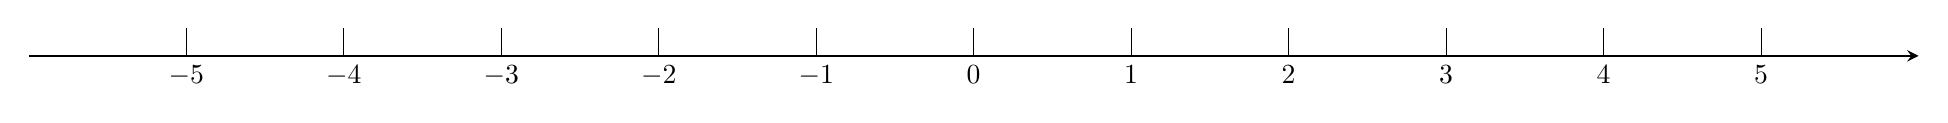
\begin{tikzpicture}[scale=2]
\draw [black, thick, ->, >=stealth] (-6,0) -- (6,0); 
\foreach \x in {-5, ..., 5}
	\draw (\x cm,5pt) -- (\x cm,0pt) node[anchor=north] {$\x$};
\end{tikzpicture}
\end{figure}
\end{frame}

\begin{frame}{最简数轴}
\begin{definition}
\textbf{\textcolor{orange}{规定了原点、正方向和单位长度的直线叫做数轴(number axis).} } \\
\end{definition}
\vspace{12pt}
\vspace{1cm}
\textbf{以下图形是不是一个数轴?}
\vspace{1cm}
\begin{figure}
\fontsize{20}{24}\selectfont
\begin{tikzpicture}[scale=2]
\draw [black, thick, -stealth] (-4,0) -- (4,0); 
\foreach \x in {0, 1}
 	\draw (\x cm,5pt) -- (\x cm,0pt) node[anchor=north] {$\x$};
\end{tikzpicture} 
\end{figure}
\end{frame}

\begin{frame}{类比思维}
\textbf{\textcolor{orange}{规定了原点、正方向和单位长度的直线叫做数轴(number axis).} } 
\begin{figure}
\fontsize{20}{24}\selectfont
\begin{tikzpicture}

\coordinate (A) at (-5, 0);
\coordinate (B) at (-3, 0);
\coordinate (C) at (-2, 0);
\coordinate (D) at (2,0);
\coordinate (D1) at (5, 0);

\coordinate (E1) at (-5, -2);
\coordinate (F1) at (5, -2);
\coordinate (E) at (-2, -2);
\coordinate (F) at (2, -2);
\draw [Circle-Circle] (A) node [below] {A} -- node [above =0.1cm] {线段AB} (B) [below] node {B}; %画线段
%画射线
\draw [Circle-] (C) node [below] {C} -- node  [above=0.1cm] {射线CD}  (D1);
\fill (D) circle(2pt) node [below] {D}; 
 %画直线
\draw (E1)  --node  [above=0.1cm] {直线EF} (F1);
\fill (E) circle(2pt) node [below] {E}  (F) circle(2pt) node [below] {F};

\end{tikzpicture}
\end{figure}
【北京师范大学四年级上册(2013)P16】\\
\textbf{线段:线段有两个端点,线段有一定的长度。} \\
\textbf{射线:射线有一个端点,射线可以向一个方向无限延伸。} \\
\textbf{直线:直线没有端点,直线可以向两个方向无限延伸。} \\
\begin{figure}
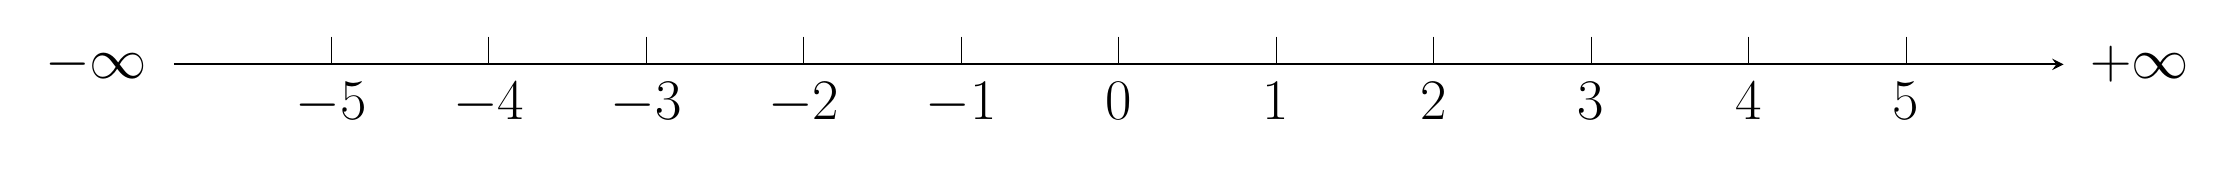
\begin{tikzpicture}[scale=2]
\fontsize{20}{24}\selectfont
\draw [black, thick, -stealth] (-6,0) node [left=0.1cm] {$-\infty$} -- (6,0) node [right=0.1cm] {+$\infty$}; 
\foreach \x in {-5,...,5}
 	\draw (\x cm,5pt) -- (\x cm,0pt) node[anchor=north] {$\x$};
\end{tikzpicture} 
\end{figure}
\textbf{实数集$\mathbb{R}$可以用区间表示为$(-\infty, +\infty)$,$\infty$读作“无穷大”,“$-\infty$”读作“负无穷大”,“$+\infty$”读作“正无穷大”.【必修A版一册P64】}
\end{frame}

\end{document}
% 1.3 相反数
\begin{frame}{1.3 相反数}
\begin{definition}
\textbf{\textcolor{orange}{只有正负号不同的两个数称互为相反数(opposite number)。\\
我们规定: 0 的相反数是0 .}}
\end{definition}
\begin{columns}
\column{0.5\textwidth}
\begin{itemize}
    \item \textbf{数学表达式}:  $a + b = 0$
    \item \textbf{函数定义}:  $f(x) = -x$
    \item \textbf{定义域}: $x \in \mathbb{R}$
    \item \textbf{值域}: $y \in \mathbb{R}$
    \item \textbf{对称性}: 关于原点中心对称
\end{itemize}

\column{0.5\textwidth}
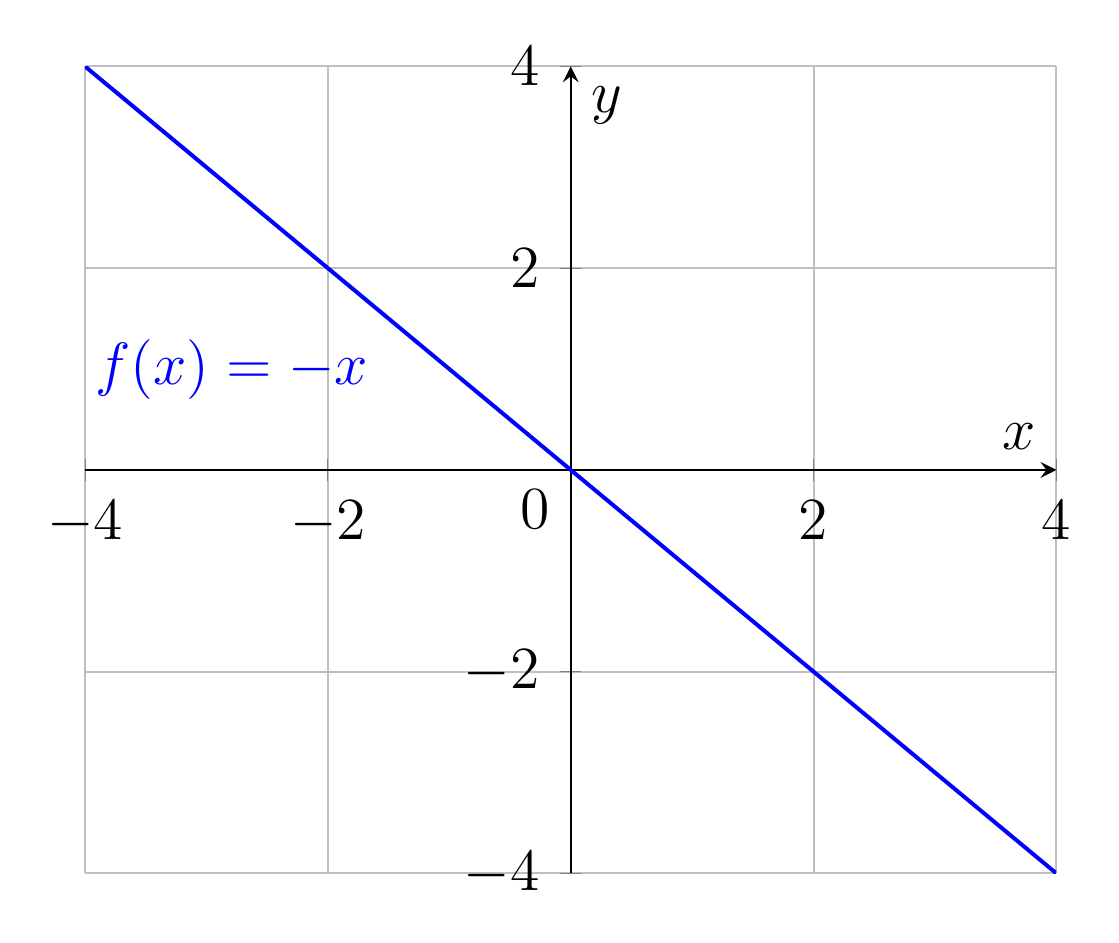
\begin{tikzpicture}[scale=1.8]
\fontsize{12}{14}\selectfont
\begin{axis}[
    axis lines=middle,
    xlabel=$x$, ylabel=$y$,
    xmin=-4, xmax=4, ymin=-4, ymax=4,
    samples=500,
    grid=both,
    restrict y to domain=-4:4,
]
\addplot[blue, thick] {-x};
\node[black] at (0,0) [below left] {0};
\node[blue] at (-1.5,1) [left] {$f(x)=-x$};
\end{axis}
\end{tikzpicture}
\end{columns}
\end{frame}

% 倒数的定义及函数图象
\begin{frame}{倒数的定义及函数图象}
\begin{definition}
\textbf{\textcolor{orange}{乘积为1的两个数互为倒数。\\
注意:0没有倒数。}}
\end{definition}
\begin{columns}
\column{0.5\textwidth}
\begin{itemize}
    \item \textbf{数学表达式}:  $a \cdot b = 1$
    \item \textbf{函数定义}:  $f(x) = \dfrac{1}{x}$
    \item \textbf{定义域}: $x \in \mathbb{R}, x \neq 0$
    \item \textbf{值域}: $y \in \mathbb{R}, y \neq 0$
    \item \textbf{对称性}: 关于原点中心对称
\end{itemize}

\column{0.5\textwidth}
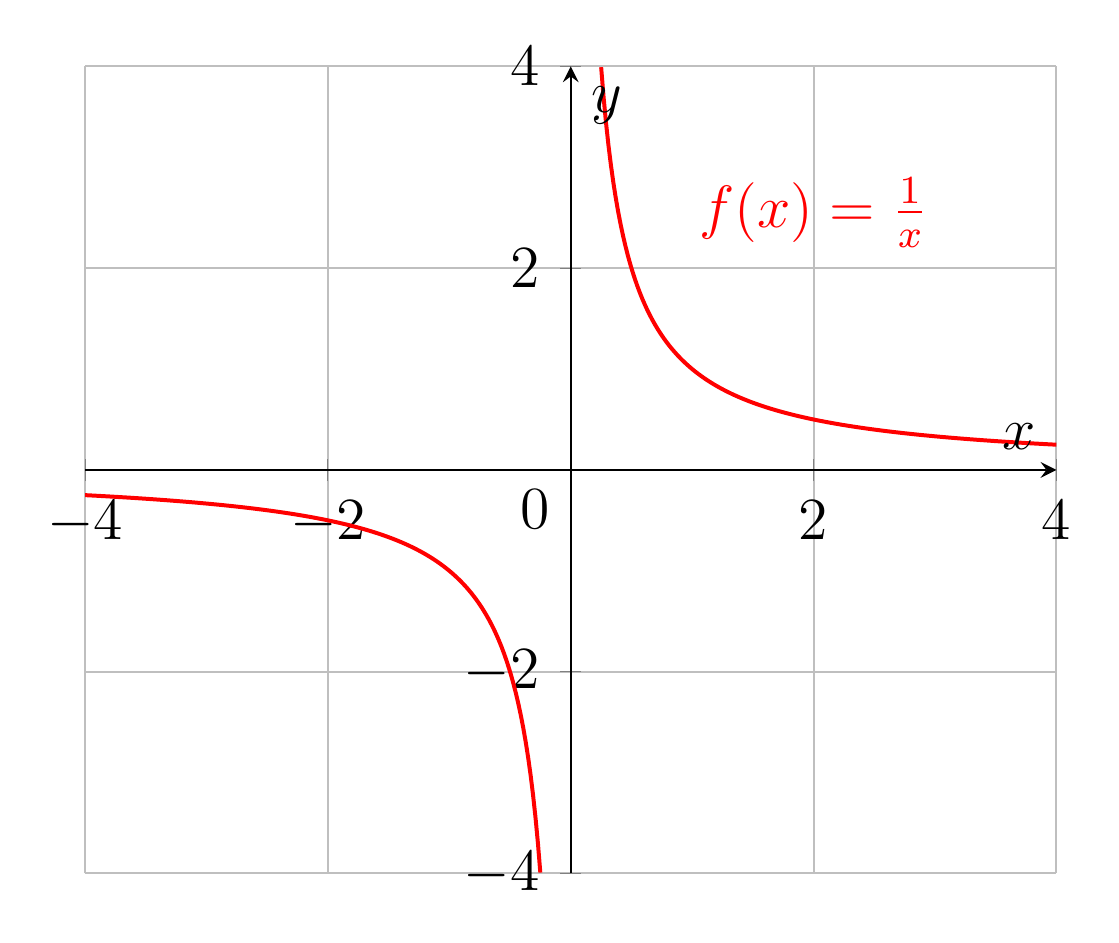
\begin{tikzpicture}[scale=1.8]
\fontsize{12}{14}\selectfont
\begin{axis}[
    axis lines=middle,
    xlabel=$x$, ylabel=$y$,
    xmin=-4, xmax=4, ymin=-4, ymax=4,
    samples=500,
    grid=both,
    restrict y to domain=-4:4,
]
\addplot[red, thick] {1/x};
\node[black] at (0,0) [below left] {0};
\node[red] at (2,2) [above] {$f(x)=\frac{1}{x}$};
\end{axis}
\end{tikzpicture}
\end{columns}
\end{frame}

% 相反数与倒数的比较
\begin{frame}{相反数与倒数的比较}
\begin{columns}
\column{0.5\textwidth}
\begin{itemize}
    \item \textbf{相反数的表达式}:  $a + b = 0$
    \item \textbf{倒数的表达式}:  $a \cdot b = 1$
    \item \textbf{对称性}: 相反数与倒数均关于原点中心对称
\end{itemize}

\column{0.5\textwidth}
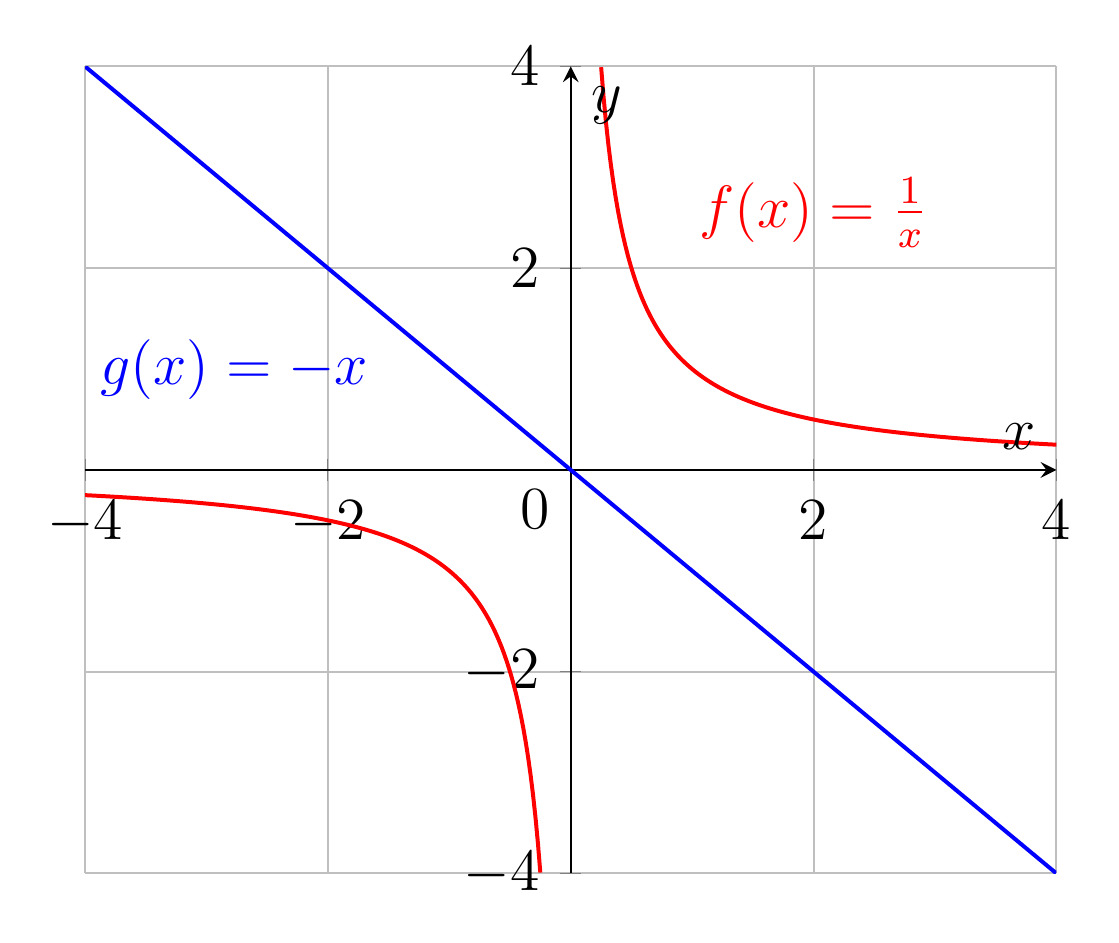
\begin{tikzpicture}[scale=1.8]
\fontsize{12}{14}\selectfont
\begin{axis}[
    axis lines=middle,
    xlabel=$x$, ylabel=$y$,
    xmin=-4, xmax=4, ymin=-4, ymax=4,
    samples=500,
    grid=both,
    restrict y to domain=-4:4,
]
\addplot[red, thick] {1/x};
\addplot[blue, thick] {-x};
\node[black] at (0,0) [below left] {0};
\node[red] at (2,2) [above] {$f(x)=\frac{1}{x}$};
\node[blue] at (-1.5,1) [left] {$g(x)=-x$};
\end{axis}
\end{tikzpicture}
\end{columns}
\end{frame}
\documentclass[aspectratio=169]{ctexbeamer} %[t]:顶端对齐
\usetheme{Madrid} %Madrid,蓝色调为主。
\usecolortheme{beaver} %beaver
\usefonttheme{professionalfonts}

\usepackage{universe}
\uBigPaper

\date{\today}
\begin{document}

% 1.4 绝对值
\begin{frame}{1.4绝对值}
\textbf{\textcolor{orange}{定义:我们把在数轴上表示数$a$的点与原点的距离叫做数$a$的绝对值, 记作|$a$|.}}
\begin{columns}
\column{0.45\textwidth}
\begin{enumerate}[label={\arabic*.}]
\item 一个正数的绝对值是它本身; 
\item 0 的绝对值是0;
\item 一个负数的绝对值是它的相反数.
\end{enumerate}

\begin{itemize}
    \item \textbf{数学表达式}:  $\left|  x  \right|$
    \item  \textbf{函数定义}: \[ f(x) = \begin{cases}
    x, x>0 \\
    0, x=0 \\
    -x, x<0
    \end{cases}
    \]
    \item \textbf{定义域}: $x \in \mathbb{R}$
    \item \textbf{值域}: $y \in \mathbb{R}, y \geq 0$
    \item \textbf{对称性}: 关于y轴对称
\end{itemize}

%绝对值函数图象
\column{0.5\textwidth}

\begin{figure}
\centering
\scalebox{1.8}{\subfile{fig/绝对值}}
\end{figure}

\end{columns}
\end{frame}

% 绝对值与相反数的比较
\begin{frame}{绝对值与相反数的比较}
\begin{columns}
%绝对值函数图象
\column{0.5\textwidth}
\textbf{绝对值的函数图象} \\
\begin{figure}
\centering
\scalebox{1.8}{\subfile{fig/绝对值}}
\end{figure}

%相反数函数图象
\column{0.5\textwidth}
\textbf{相反数的函数图象} \\
\begin{figure}
\centering
\scalebox{1.8}{\subfile{fig/相反数}}
\end{figure}

\end{columns}
\end{frame}

\end{document}

\documentclass[aspectratio=169]{ctexbeamer} %[t]:顶端对齐
\usetheme{Madrid} %Madrid,蓝色调为主。
\usecolortheme{beaver} %beaver
\usefonttheme{professionalfonts}

\usepackage{universe}
\uBigPaper

\date{\today}
\begin{document}

% 1.5 有理数的代销比较
\begin{frame}[t]{1.5有理数的大小比较规则}
\large
\begin{enumerate}[label={\arabic*.}]
  \item 数轴上右边的数比左边的数\alert{大}
  \item 正数 \alert{>} 0
  \item 负数 \alert{<} 0
  \item 正数 \alert{>} 负数
  \item 两个负数比较,绝对值大的反而\alert{小} !
  \par 如果$a > b$,则:$-a < -b$
\end{enumerate}

\end{frame}

\begin{frame}[t]{数轴比较法}
\large
\begin{enumerate}[label={\arabic*.}]
  \item 画数轴并标出所有数
  \begin{figure}
  \begin{tikzpicture}[scale=2]
  \fontsize{16}{20}\selectfont
  \draw [black, thick, ->, >=stealth] (-6,0) -- (6,0); 
  \foreach \x in {-5, ..., 5}
  	\draw (\x cm,5pt) -- (\x cm,0pt) node[anchor=north] {$\x$};
    \fill [blue] (-2,0) circle(2pt) node [above=0.3cm] {$a$};
    \fill [blue] (3,0) circle(2pt) node [above=0.3cm] {$b$};    
  \end{tikzpicture}
  \end{figure}
  \item 从左到右(从小到大)排列
  \item 结果:$a \alert{<} b$
\end{enumerate}

\end{frame} 

\end{document}

\end{document}